\section{Methodology}
To understand the flow behaviour in various undertray geometries, some kind of analysis of the fluid dynamics is required. The rapid development of computational power has allowed more accurate and reliable computational analysis results such as computational fluid dynamics (CFD) \cite{Andersson2011ComputationalEngineers}. The usage of CFD allows engineers to simplify design processes and to achieve an accurate flow prediction in a relatively short period of time, allowing engineers to do more design iterations and thus produce better designs.

\begin{figure}[!htb]
    \centering
    \makebox[\textwidth]{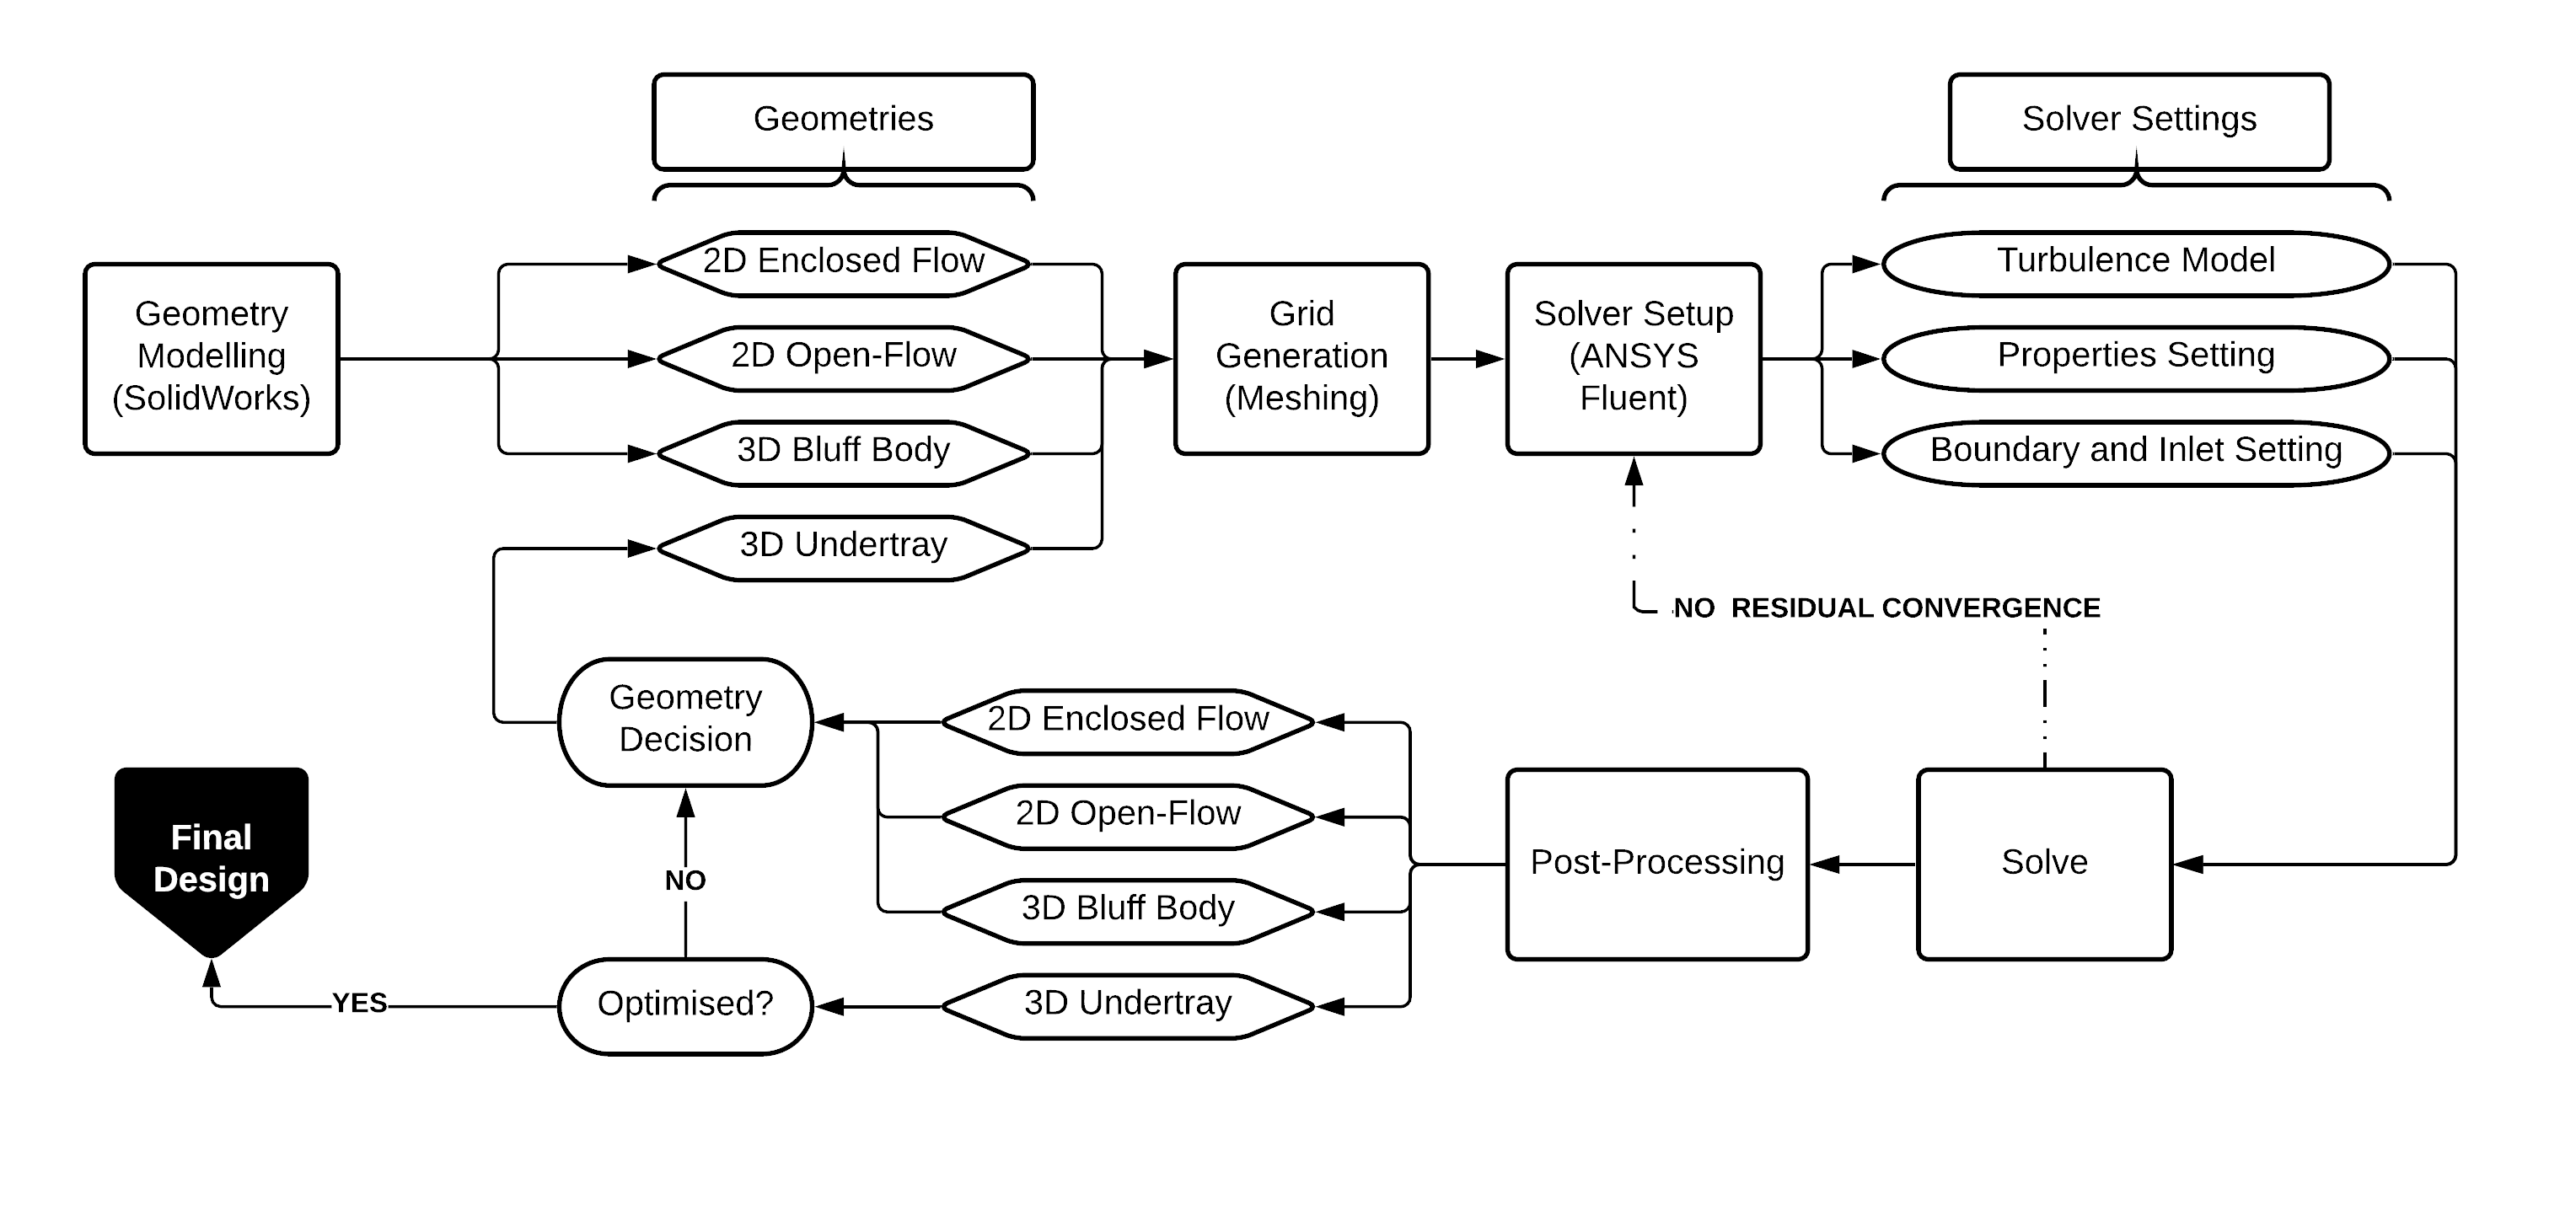
\includegraphics[scale=0.15]{Figures/project_methodology_chart.png}}
    \caption{Project Methodology Flow Chart}
    \label{fig:project methodology}
\end{figure}

\noindent The methodology used in this project consists of three phases. These phases are: 2D enclosed \& open-flow; 3D bluff body flow, 3D full undertray flow. The first phase consists of 2D analysis, which analyses the undertray variables on a Venturi-tube like geometry, and open-flow analysis to determine the effect of a simple bluff body with similar undertray variables. The 3D bluff body phase takes the 2D geometry, extrudes it into a 3D geometry, and then analyses it. Lastly is the 3D full undertray, in which the results from previous analysis will be used to optimise the final undertray design's geometry. A simplified traced body from the QFR 2021 car will be attached to the undertray to achieve results without the geometrical complexity of the full CAD model. The full workflow of the process is illustrated in Figure~\ref{fig:project methodology}. This project will be entirely computationally based, and makes use of ANSYS Fluent as the default working platform.

\subsection{Pre-Processing \& Solver Setup}

\subsubsection{Grid Generation (Meshing)}
\noindent The surfaces or bodies which have been defined from the SolidWorks CAD model forms the basis for the meshing. The meshing program, which is integrated with ANSYS Workbench, provides a user-friendly, simple, and fast mesh generator. Due to the constraints on computational power and time, unstructured triangular (2D) and tetrahedral (3D) mesh were mostly used, with quadrilaterals (2D) and triangular prisms (3D) used near the wall as an inflation layer to capture the growth of the boundary layer and reduce numerical diffusion \cite{Lanfrit2005BestFLUENT}.

\noindent The goal of the 2D and 3D bluff body simulations is to obtain and analyse the trend in performance resulting from changes to the undertray geometry; therefore, a simple yet high quality mesh could be generated in an unstructured manner. Local refinement around the solid body is recommended \cite{Lanfrit2005BestFLUENT} to achieve reasonable results and representation of the flow, especially around the undertray. Moreover, this technique allows reduced mesh density in the far-field sections less likely to be affected by or affecting the result. Another aspect of quality meshing is the mesh metrics such as skewness and growth ratio. For automotive applications, it is recommended to have skewness less than 0.45 and a maximum growth rate of less than 20\% \cite{Lanfrit2005BestFLUENT}. 

\noindent One crucial factor in an undertray flow is the development of the boundary layer and how this interacts with the moving floor. The accuracy of this aspect is dependent on the quality of the grid near the wall, and on the wall function being used. To generate a high quality inflation layer, it is essential to make sure the y+ value (first layer grid height) does not exceed the inner boundary layer region, which can be calculated using the expression:

\begin{equation}
    y^+ = \frac{\rho U_\tau \partial y}{\mu}, where \quad U_\tau = \sqrt{\frac{\tau_w}{\rho}} = U \sqrt{\frac{1}{2}C_f}
\end{equation}

\noindent Figure~\ref{fig:inflation layer} shows an illustration of the relevance of the $y^+$ value close to a wall. The turbulence model being used by the solver also has to be considered in defining the required $y^+$ value. Some turbulence modelling requires a very low $y^+$, whereas some can tolerate higher values. The detail of $y^+$ value in the various turbulence models will be discussed in the next section. 

\begin{figure}[!ht]
    \centering
    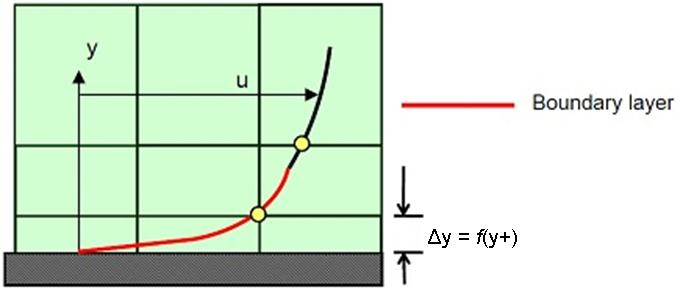
\includegraphics[height=4cm]{Figures/inflation_layer.jpg}
    \caption{Representation of grid y+ close to a viscous wall \cite{Anonymous2013Inflate4Blog}.}
    \label{fig:inflation layer}
\end{figure}


\subsection{Numerical Method}
\noindent The turbulence model is a crucial aspect in approximating the effect of unsteady turbulent fluctuations on the flow \cite{Cummings2015AppliedAerodynamics}. The quality of the turbulence modelling can significantly impact the fidelity of the simulations \cite{Lanfrit2005BestFLUENT}. Due to the time constraints and limited computational resources available for this project, a steady-state method was used throughout. To account for the effects of turbulence, a two-equation Reynolds-Averaged Navier-Stokes (RANS) approach was used to solve the time-averaged flow \cite{Cummings2015AppliedAerodynamics}. With a reasonable quality of mesh, physical lift and drag trends can be predicted, which can then be studied. The Realizable $k-\epsilon$ and $k-\omega$ Shear Stress Transport (SST) models were used in this project to solve the equations and estimate the downforce and drag of the undertray and bluff body.  

\subsubsection{Realizable $k-\epsilon$ Models}
The $k-\epsilon$ turbulence model is a two-equation transport model which specifically solves equations for the turbulence kinetic energy ($k$) and turbulence dissipation rate ($\epsilon$) \cite{Andersson2011Turbulent-flowModelling} \cite{Mansour1989Near-wallModeling} \cite{Ansys2006ModelingFlows}. The standard model is robust and widely used across a broad swathe of applications in engineering turbulence modelling; however, the nature of $k-\epsilon$ family is not able to calculate some of the $\epsilon$ terms which can be anticipated using wall function. Moreover, k-$\epsilon$ does not perform well for flow with strong separation and large adverse pressure gradient, which the primary feature of an undertray's diffuser \cite{Ansys2006ModelingFlows}.  Therefore realisable k-$\epsilon$ is broadly used in this analysis. The term 'realisable' itself allows some of the mathematical satisfaction in computing the Reynolds stresses, improving its turbulent flow consistency. This specific transport model is crucial to capture important flow features of an undertray, such as flow rotation, significant adverse pressure gradient, and vortex formation.
\begin{align}
\frac{\partial}{\partial t}(\bar{\rho} k)+\frac{\partial}{\partial x_j}(\bar{\rho} \tilde{u}_j k) & = \frac{\partial}{\partial x_j} \left[ \left(\mu + \frac{\mu_t}{\sigma_k}\right) \frac{\partial k}{\partial x_j} \right] +P_k-\bar{\rho}\epsilon \\ 
\frac{\partial }{\partial t}(\bar{\rho} \epsilon)+\frac{\partial}{\partial x_j}(\bar{\rho} \tilde{u}_j \epsilon) & = \frac{\partial}{\partial x_j} \left[ \left(\mu + \frac{\mu_t}{\sigma_{\epsilon}}\right) \frac{\partial \epsilon}{\partial x_j} \right] + \frac{\epsilon}{k}(C_{\epsilon 1}P_k-C_{\epsilon 2}\bar{\rho} \epsilon),
\end{align} 

\subsubsection{$k-\omega$ Shear Stress Transport (SST) Models}
The SST model is another two equation-model. It combines both the $k-\epsilon$ and $k-\omega$ models \cite{Andersson2011Turbulent-flowModelling}\cite{Ansys2006ModelingFlows}.  The $k-\epsilon$ approach is used in the free-stream, and $k-\omega$ is used near the boundary surface, meaning that this model takes the strength of, theoretically allowing accurate predictions in all regions. This model is known to perform well in regions with adverse pressure gradients and with flow separation; moreover, SST is known to have more accurate performance in the boundary layer compared to $k-\epsilon$ and does not require any wall function\cite{Andersson2011Turbulent-flowModelling}. However, a fine mesh ($y^+  < 5$) is required near the wall, which increases the computational cost and time, and it can over-predict turbulence levels flow in high strain areas \cite{Andersson2011Turbulent-flowModelling}\cite{Ansys2006ModelingFlows}. \begin{align}
\frac{\partial }{\partial t}({\rho} k)+\frac{\partial}{\partial x_j}({\rho} {u}_j k) & = \frac{\partial}{\partial x_j} (\Gamma_{k} \frac{\partial k}{\partial x_j}) + \tilde{G_k} - Y_k +s_k \\
\frac{\partial}{\partial t}(\rho \omega)+\frac{\partial}{\partial x_j}({\rho} {u}_j \omega) & = \frac{\partial}{\partial x_j}(\Gamma_\omega \frac{\partial \omega}{\partial x_j}) + G_\omega - Y_\omega + D_\omega + S_\omega
\end{align} 

\subsection{Boundary Conditions}
\begin{table}[!htb]
\centering
    \caption{Boundary Conditions for 2D and 3D ANSYS Fluent setup}
    \label{tab:Boundary Conditions}
\begin{tabular}{||p{3cm}|p{3cm}|p{6cm}||}
 \hline
 \centering
 Named Region  &  Boundary Condition  & Property Details\\
 \hline \hline
 \multicolumn{3}{||c||}{General Properties} \\
 \hline
 
 Inlet & Inlet velocity & Velocity = 16.667 m/s (or 40 km/h)\\
 \hline
 Outlet & Outlet Pressure  & Gauge Pressure = 0 Pa  \\
 \hline
 Undertray (2D Enclosed)/Bluff Body & Stationary Wall & No-slip condition\\
 \hline
 Moving Floor & Moving Wall & Velocity = 16.667 m/s (or 40 km/h) in the flow direction\\
 \hline
 Enclosure &   Fluid (Air)  & Pressure = 101325 Pa
Temperature = 288.15 K
Density = 1.225 kg/m3
ISA Sea Level Condition\\
 
 \hline
 \multicolumn{3}{||c||}{3D Analyses} \\
 \hline
 
 Symmetry Body & Symmetry  & -\\
 \hline
 Symmetry Top & Symmetry  & -\\
 \hline
 Symmetry Side & Symmetry & -\\
 \hline
 
\end{tabular}
\end{table}

\noindent Table \ref{tab:Boundary Conditions} shows the boundary conditions that were used for both the 2D and 3D analyses in the ANSYS Fluent solver. The main goal of these simulations is to simulate the flow behaviour at the bottom region of the car; therefore, a moving floor was employed in all simulations, with the same magnitude and direction as the oncoming flow. The use of a moving ground condition (or a belt in a wind tunnel) is physically correct, and represents the best option for capturing the ground effect in such an undertray \cite{Zhang2006GroundCars}\cite{Burgin1986WINDEFFECT}. The simulation environment was set from the International Standard Atmospheric (ISA) conditions at sea level. 

\noindent In the three dimensional simulations, the side, far-side, and the top surface of the flow-field were set to symmetry conditions, in which the fluxes and normal gradients of all the variables are assumed zero \cite{ANSYS2009SymmetryConditions}, as recommended by Lanfrit \cite{Lanfrit2005BestFLUENT}. Along with the moving floor, this setup was considered to provide the best results and nearest approximation to simulating the behaviour of a race car on an actual racing track.





